\section{Case Study}
We have developed an open-source tool dReach using OCaml to perform $\delta$-complete reachability analysis for hybrid systems \cite{dreach}. dReach is built upon our SMT solver dReal \citep{dreal} that implements a $\delta$-complete decision procedure. To exemplify different aspects of our parameter synthesis framework, we carried out a case study on the electrical dynamics of cardiac cells. All the experiments reported below were done using a machine with two Intel Xeon E5-2650 2.00GHz processors and 64GB RAM. The precision was set to be $0.001$.

\begin{figure}[t]
\centering
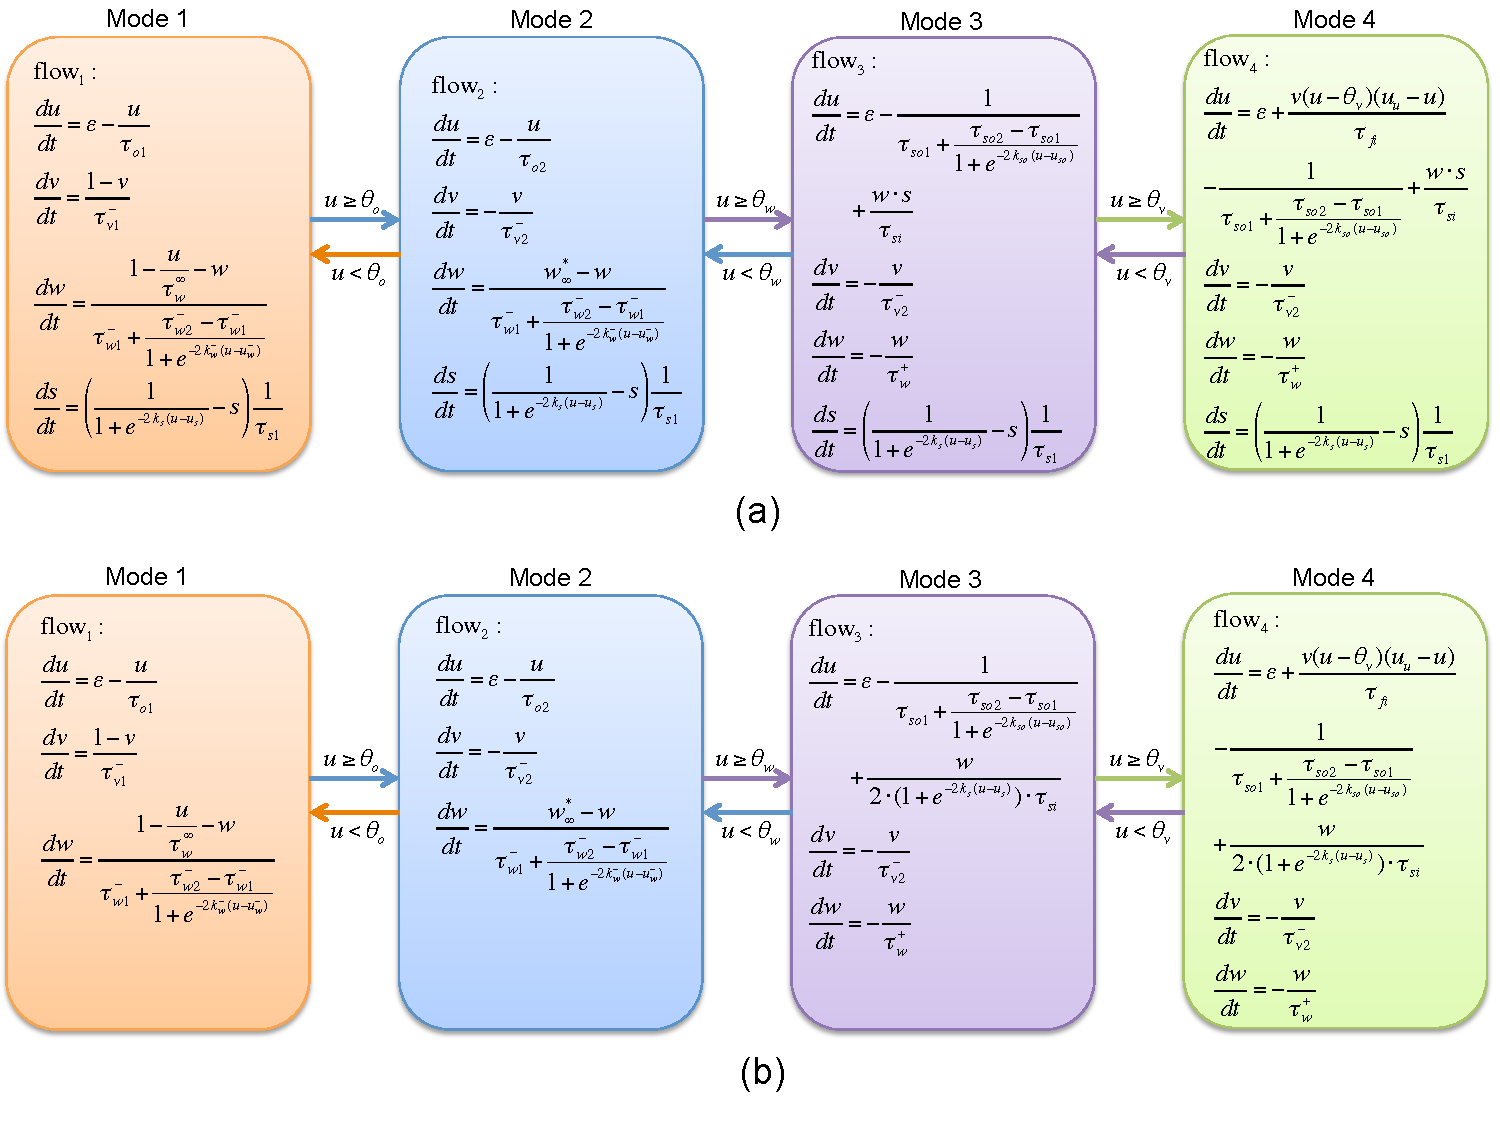
\includegraphics[scale=0.5]{fig-cardiac-new}
\caption{Hybrid models of cardiac cells. (a) BCF model. (b) FK model.}
\label{model}
 %\vspace{-0.7cm}
\end{figure}

\subsection{Hybrid models of cardiac cells}
Heart rhythm is enabled by the electrical activity of cardiac muscle cells, which make up the atria and ventricles. The electrical dynamics of cardiac cells are governed by the organized opening and closing of ion channel gates on the cell membrane. Improper functioning of the cardiac cell ionic channels can cause the cells to lose excitability, which disorders electric wave propagation and leads to cardiac abnormalities such as ventricular \textit{tachycardia} or \textit{fibrillation}. Hybrid automata models has been developed recently in order to understand the mechanisms of cardiac disorders, including the Fenton-Karma (FK) model \cite{fenton98} and the Bueno-Cherry-Fenton (BCF) model \cite{orovio08}. 

\paragraph{BCF Model.} 
In BCF the change of cell�s transmembrane potential $u$, in response to external stimulus $\epsilon$ from neighboring cells, is regulated by a fast ion channel gate $v$ and two slow gates $w$ and $s$.
Figure \ref{model}(a) shows the four modes associated with BCF. In Mode $1$, gates $v$ and $w$ are open and gate $s$ is closed. The transmembrane potassium current causes the decay of $u$. The cell is resting and waiting for stimulation. We assume external stimulus $\epsilon$ equals to $1$ and lasts for $1$ millisecond. The stimulation causes $u$ increase, which may trigger $\jump_{1 \rightarrow 2}: u \geq \theta_o$. In Mode 2, $v$ starts closing. The decay rate of $u$ changes. The systems will jump to Mode 3 if $u \geq \theta_w$. In Mode 3, $w$ is also closing. $u$ is governed by the potassium current and the calcium current. When $u \geq \theta_v$, Mode 4 can be reached which means a successful AP initiation. In Mode 4, $u$ reaches its peak due to the fast opening of sodium channel. The cardiac muscle contracts and $u$ starts decreasing. 

\paragraph{FK Model.} 
As shown in Figure \ref{model}(b), FK comprises the same four modes and equations of BCF except that the current change induced by gate $s$ is reduced to an algebra function, which is integrated to $du/dt$. Similar to BCF, an AP can be successfully initiated when Mode 4 is reached. 


We specified BCF and FK using dReach language. Starting from the state ($u = 0$, $v = 1$, $w = 1$, $s = 0$) of Mode 1, we checked whether Mode 4 is reachable using the parameter values presented in \cite{orovio08}. $\mathsf{sat}$ was returned for both BCF and FK. Witness trajectories were simulated and shown in Figure \ref{trace} (the stimulus $\epsilon$ was reset every $500$ milliseconds).


\begin{figure}[thb]
\centering
\subfigure[]{
  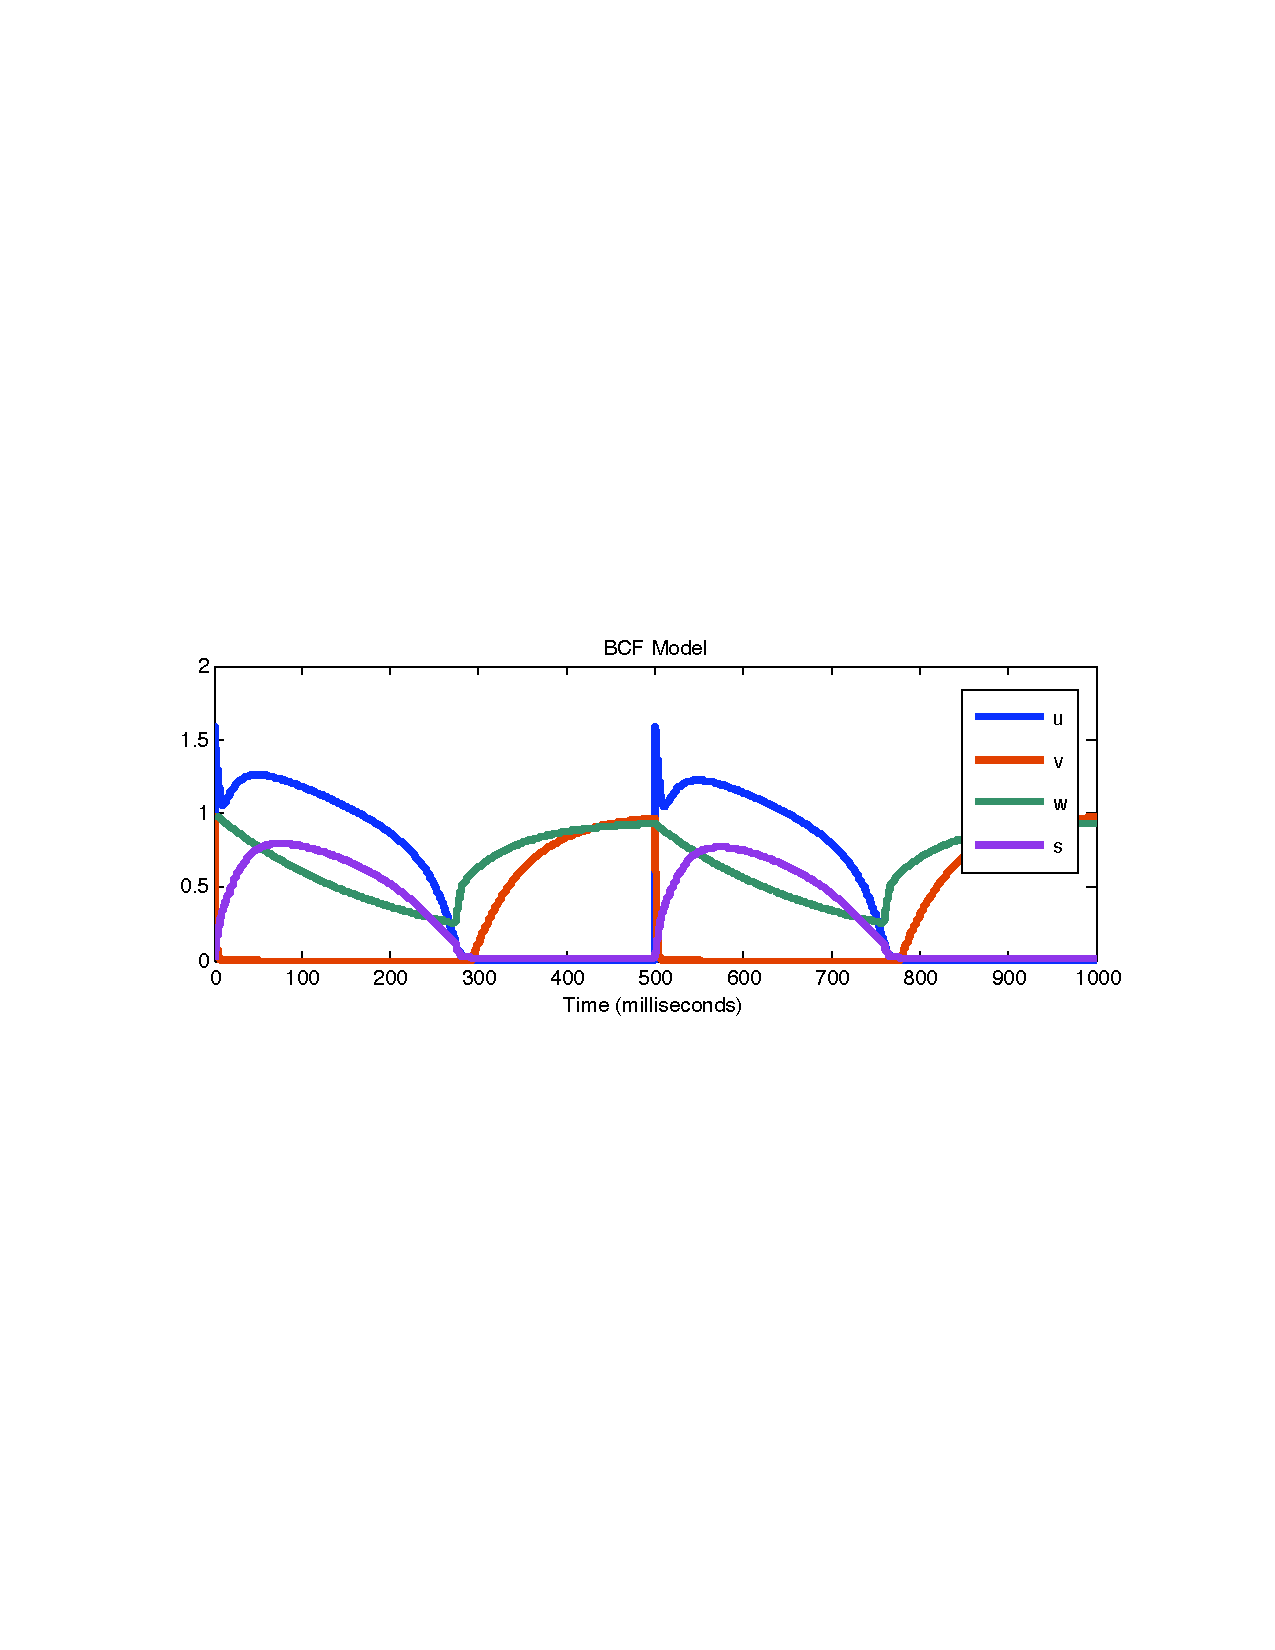
\includegraphics[width=8cm]{fig-bcf}
} 
\subfigure[]{
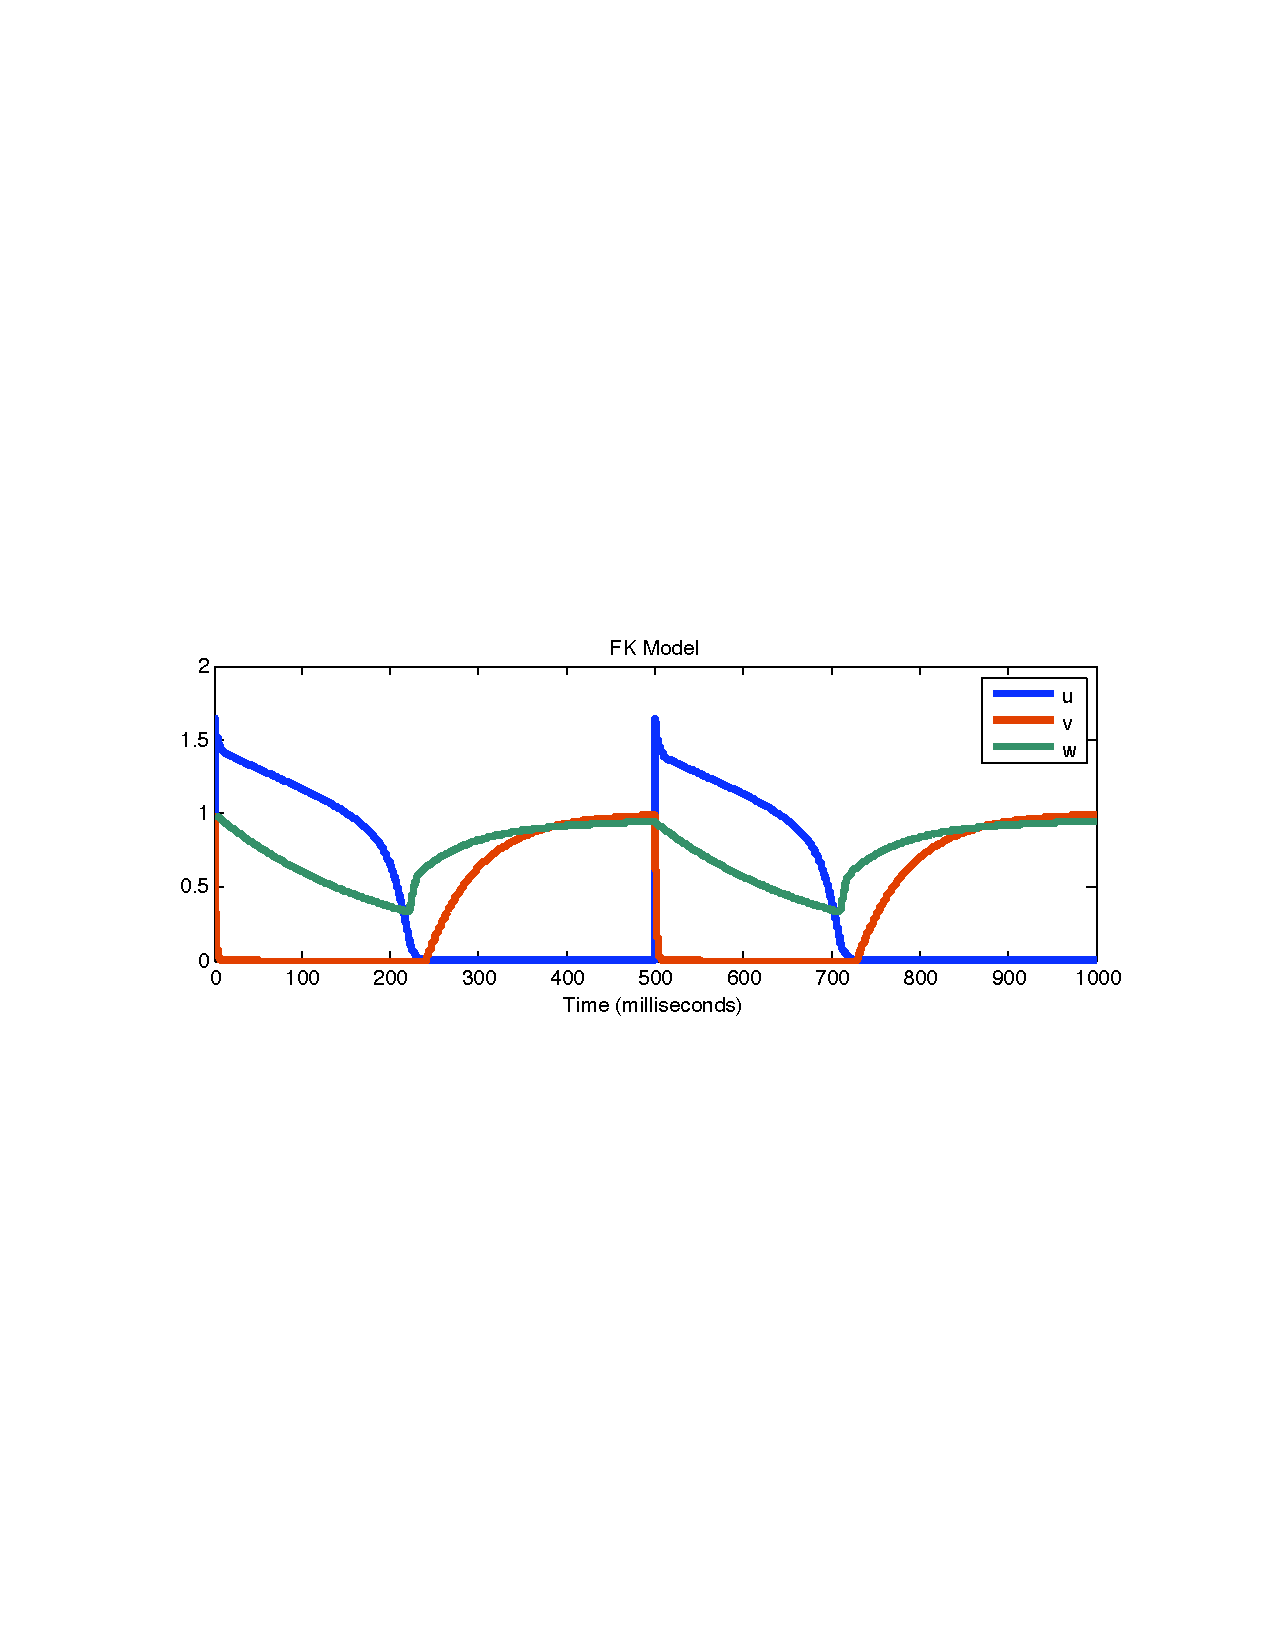
\includegraphics[width=8cm]{fig-fk}
}
\caption{The simulated time profile of BCF and FK.}
\label{trace}
 %\vspace{-0.7cm}
\end{figure}


\subsection{Model falsification}
BCF and FK were able to reproduce essential characteristics (e.g. steady-state action potential duration) observed in human ventricular cells \cite{fenton98,orovio08}. However, ventricular cells comprised three cell types, which possess different dynamical characteristics. For instance, Figure \ref{ap} shows that time courses of action potentials (APs) for epicardial and endocardial human ventricular cells have different morphologies \cite{nabauer96}. An important \textit{spike-and-dome} AP morphology can only be observed in epicardial cells but not endocardial cells. Hence, in a model-based study, one needs to identify cell-type-specific parameters to take account into cellular heterogeneity. The feasibility of this task will depend on the model of choice, as certain model would be impossible to reproduce a dynamical behavior no matter which parameter values are used. Here we illustrate that such models can be ruled out efficiently using our $\delta$-decision based parameter synthesis framework.

\paragraph{Robustness.} 
To ensure proper functioning of cardiac cells in noisy environments, an important property of the system is to filter out insignificant stimulation. Thus, we expected to see that APs could not be initiated for small $\epsilon$. Starting from the state ($u = 0$, $v = 1$, $w = 1$, $s = 0$, $\epsilon \in [0.0,0.25]$) of Mode 1, we checked the reachability of Mode 4. $\mathsf{unsat}$ was returned for both BCF and FK, showing that the two models are robust to stimulation amplitude.

\begin{figure}[th]
\centering
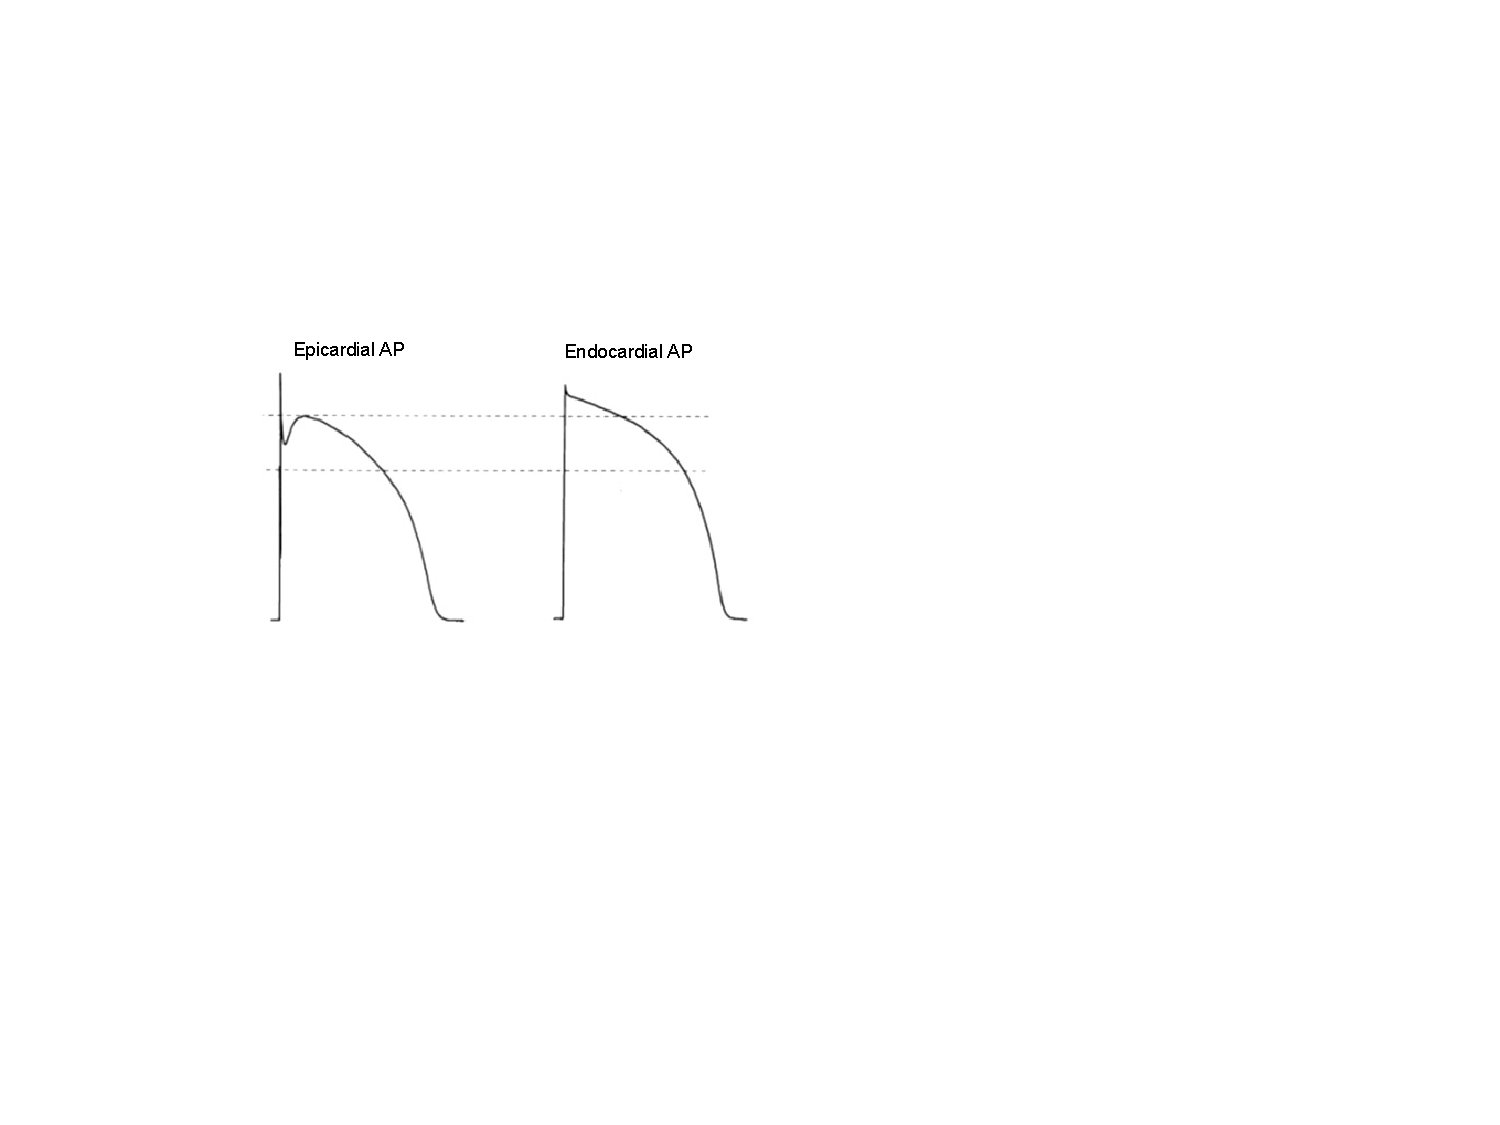
\includegraphics[scale=0.8]{fig-ap}
\caption{Experimental AP morphology \cite{nabauer96}.}
\label{ap}
 %\vspace{-0.7cm}
\end{figure}

\paragraph{AP morphology.}
Next we tested whether BCF and FK can reproduce the spike-and-dome AP morphology of epicardial cells. We introduced two auxiliary modes (Modes 5 and 6). The system will jump from Mode 4 to Mode 5 if $\tau \le 10$, and will jump from Mode 5 to Mode 6 if $\tau \le 30$. In Modes 5 and 6, we enforced invariants $1.0 \le u \le 1.15$ and $1.18 \le u \le 2.0$, respectively, to depict the spike-and-dome morphology observed experimentally \cite{nabauer96}. We then checked the reachability of Mode 6, starting from Mode 1 at state ($u = 0$, $v = 1$, $w = 1$, $s = 0$, $\epsilon \in [0.9,1.1]$, $\tau_{si} \in [1,2]$, $u_s \in [0.5,2]$). $\mathsf{sat}$ was returned for BCF, while $\mathsf{unsat}$ was returned for FK, indicating that FK is impossible to reproduce spike-and-dome shapes using reasonable parameter values. Hence FK is not suitable to study the dynamics of epicardial cells.



\subsection{Parameter identification for cardiac disorders}

When the system cannot reach Mode 4, the cardiac cell loses the excitability, which might lead to tachycardia or fibrillation. Starting with Mode 1, our next goal was to identify parameter ranges using which the system will never go into Mode 4. In what follows, we focused our study on BCF. 

\cite{grosu11} has tackled this parameter identification problem by linearizing BCF into a piecewise-multiaffine system (referred as MHA). Due to the simplification, parameter ranges could be identified using the Rovergene tool \cite{rovergene}. However, BCF and MHA have different sets of parameters. Here we aimed to identify disease-related ranges of original BCF parameters. It can be derived from equations that $\tau_{o1}$ and $\tau_{o2}$ govern the dynamics of $u$ in Mode 1 and Mode 2 respectively, and hence determine whether $\jump_{1\rightarrow 2}$ and  $\jump_{2\rightarrow 3}$ can be triggered. For $\tau_{o1}$, we performed a binary search in value domain $[0.0001,0.01]$ to obtain a threshold value $\theta_{o1}$ such that Mode 4 is unreachable if $\tau_{o1} \in (0, \theta_{o1})$ while Mode 4 is reachable if $\tau_{o1} =  \theta_{to1}$. Specifically, for each candidate value $\theta^i_{o1}$, we checked the reachability of Mode 4 with the initial state ($u = 0$, $v = 1$, $w = 1$, $s = 0$, $\theta_{o1} = \theta^i_{o1}$). We set the next candidate to be $(\theta^i_{o1} -\theta_{l})/2$ if $\mathsf{sat}$ was returned, or $(\theta_{r} - \theta^i_{o1})/2$ if $\mathsf{unsat}$ was returned, where $\theta_{l}$ is the largest $\mathsf{unsat}$ candidate and $\theta_{r}$ is the smallest $\mathsf{sat}$ candidate. 

In this manner, we identified $\theta_{o1}$ to be $0.006$, which suggest that when $\tau_{o1} \in (0, 0.006)$, the system will always stay in Mode 1. Similarly, we also obtained a threshold value $0.13$ for $\tau_{o2}$, such that Mode 3 cannot be reached when $\tau_{o2} \in (0, 0.13)$. Furthermore, whether the system can jump from Mode 3 to Mode 4 depends on the interplay between $\tau_{so1}$ and $\tau_{so2}$.  For each value $\tau_{so2}^i$ of $\tau_{so2}$ sampled from domain $(0, 100]$, we performed the binary search in $(0, 5]$ to find the threshold value $\theta_{so1}$ such that Mode 4 is unreachable when $\tau_{so1} \in [0,\theta_{so1}]$ and $\tau_{so2} = {\tau_{so2}^i}$. By linear regression of the obtained values of $\theta_{so1}$, we identified one more condition that Mode 4 is unreachable:  $6.2 \cdot \tau_{so1} + \tau_{so2} \ge 9.9$. Token together, we identified the following disease-related parameter ranges:  
$$\tau_{o1} \in (0,0.006)\vee \tau_{o2} \in (0,0.13)\vee 6.2 \cdot \tau_{so1} + \tau_{so2} \ge 9.9$$
Figure \ref{cresults} visualizes these results by showing the simulated trajectories using corresponding  parameter values.


\begin{figure}[h]
\centering
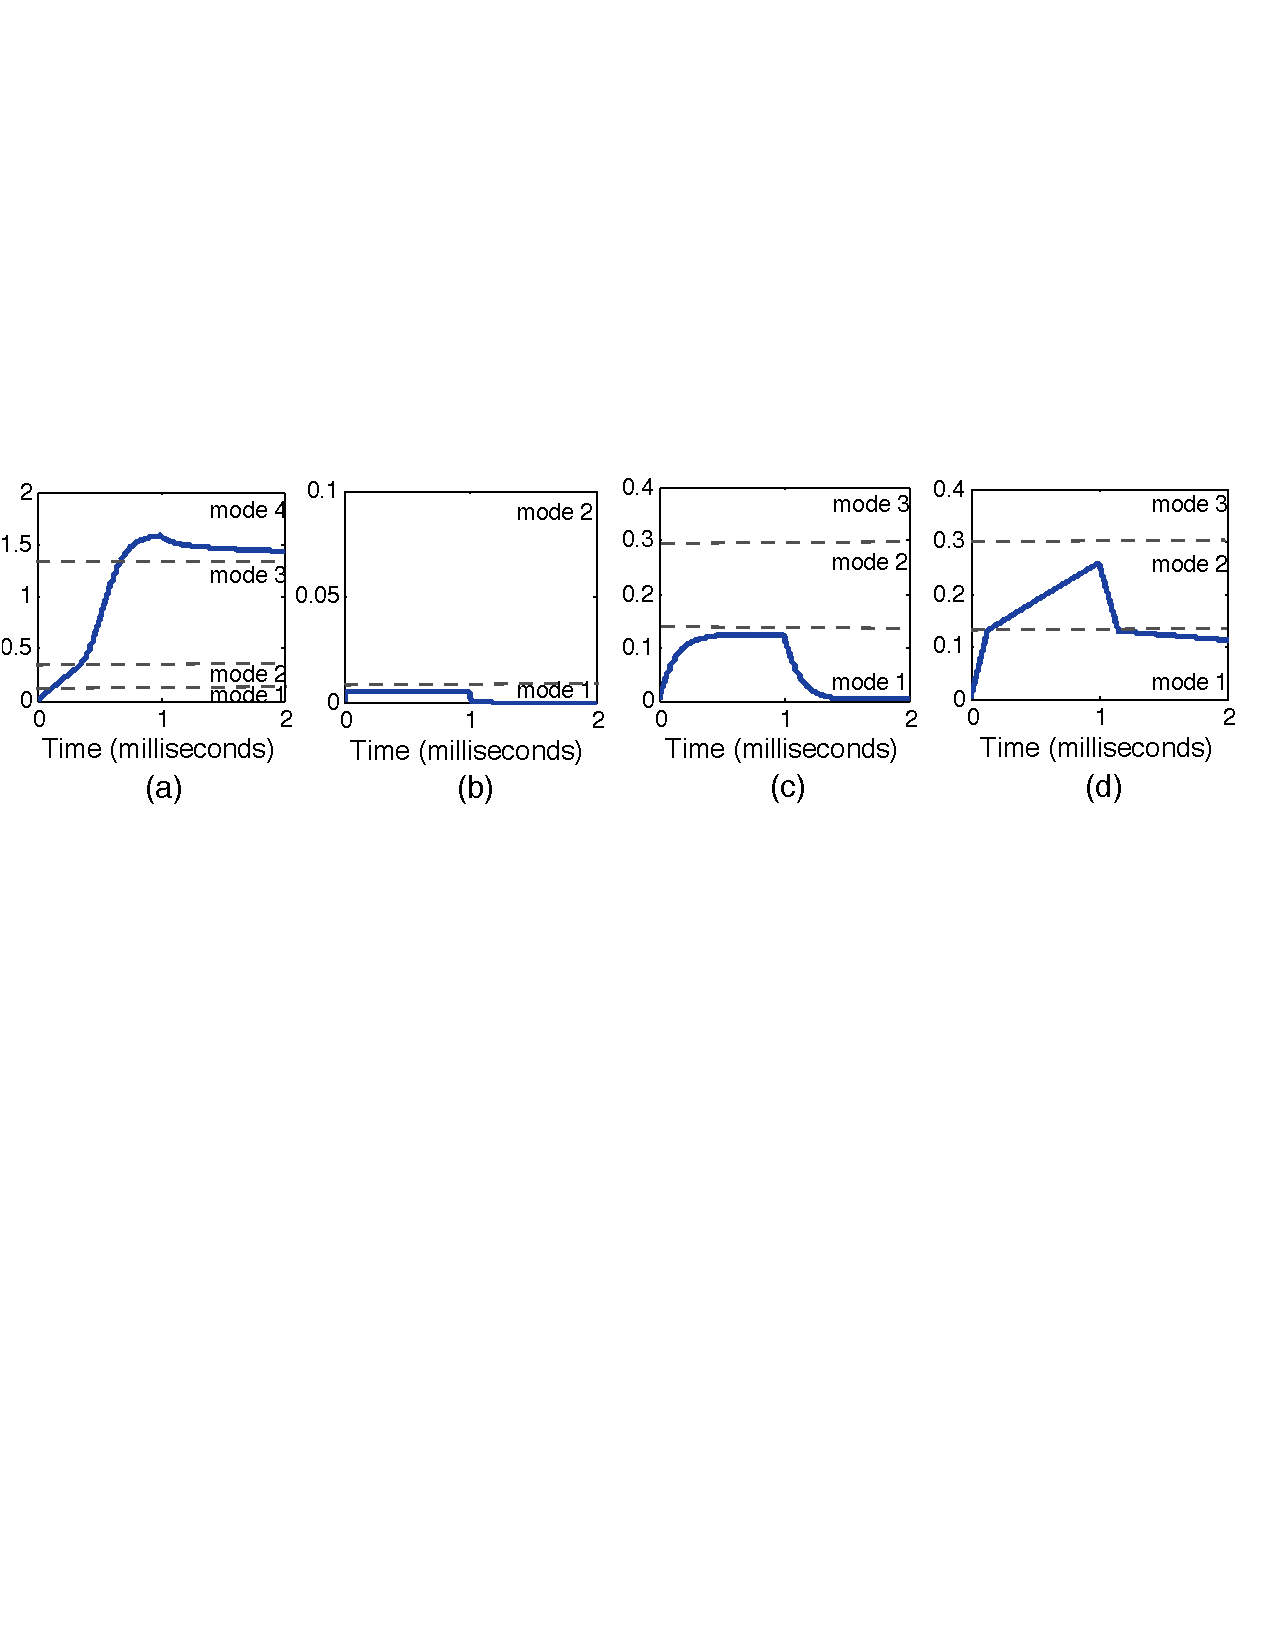
\includegraphics[scale=0.6]{fig-cardiactraj2}
\caption{Simulation results using disease related parameter values. (a) Original parameters (b) $\tau_{o1}=0.0055$ (c) $\tau_{o2} = 0.125$ (d) $\tau_{so1} =1.2$, $\tau_{so2} =1.0$ }
\label{cresults}
 %\vspace{-0.7cm}
\end{figure}

%%% Local Variables:
%%% TeX-master: "main"
%%% End:
